\section{Access methods management}

\begin{figure}[h!]
		\centering
		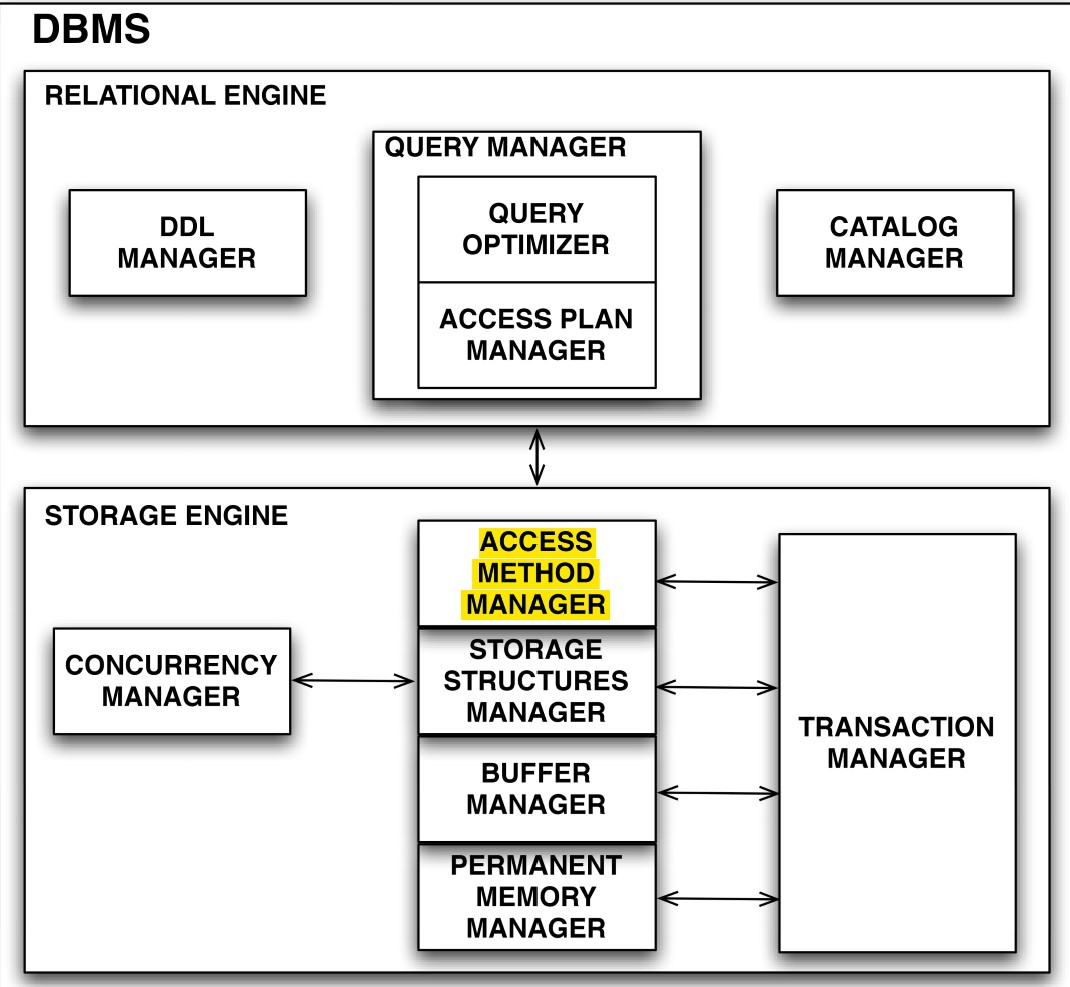
\includegraphics[scale = 0.7]{img/access1.jpg}
		\label{part6}
\end{figure}

\begin{tcolorbox}
The access method manager provides to the relational engine the operators used by its modules to execute the commands for the definition and use of DBs.
\end{tcolorbox}

\subsection{Storage engine}
A DBMS is typically divided into:

\begin{itemize}
    \item the \textbf{relational engine}, which includes modules to support the execution of SQL commands and interacts with the storage engine;
    \item the \textbf{storage engine}, which includes modules to execute the operations on data stored in the permanent memory.
\end{itemize}

Normally, the storage engine is not accessible to the user, who will interact with the relational engine.

While the interface of the relational engine depends on the data model features, the interface of the storage engine depends on the data structures used in permanent memory. To give a better idea of the \textbf{interface of a storage engine}, we will consider the case of the relational system \textbf{JRS}, which stores relations in heap files and provides B+– tree indexes to facilitate data retrieval. The operators on data exported by the storage engine are procedural and can be grouped into the following categories:

\begin{itemize}
    \item operators to create the DBs;
    \item operators to start and end a transaction;
    \item operators on heap file and indexes;
    \item operators about access methods available (= ways of retrieving records from a table) for each relation.
\end{itemize}

We now focus on the operators on DBs, on heap files, on indexes and on the operators about access methods.

\subsection{Operators on DBs}
The operators are:
\begin{itemize}
    \item \textit{createDB}, which creates a DB in the specified path;
    \item \textit{createHeapFile}, which creates an heap file in the DB in the specified path;
    \item \textit{createIndex}, which creates an index on a relation attribute, which could be a key, or on multiple attributes.
\end{itemize}

A DB, an heap file or an index can be deleted using \textit{dropDB}, \textit{dropHeapFile} and \textit{dropIndex}

\subsection{Operators on heap files}
A DB table is stored in a heap file, in which there are operators to insert, delete, retrieve or update records with a specified RID, or to get the number of pages used and the number of the record. A \textbf{table} is a set of records where each record contains the same number of fields. Heap files support the \textit{scan} operation to iterate through the records of a file.

\subsection{Operators on indexes}
An index is a set of records (Value, RID), organized as a B+-tree: the Value is the search key, while RID is the identifier of the record with the search key Value. Any number of indexes can be defined on a relation, and a search key can be multi-attribute. The operators available on indexes are those to insert or delete elements, or to get data about the B+–tree used to store them, such as the number of leaves, minimum and maximum search key Value.

\subsection{Access methods operators}

\begin{tcolorbox}
    The Access Methods Manager provides the operators to transfer data between permanent memory and main memory in order to answer a query on a database. 
\end{tcolorbox}

Permanent data are organized as collections of records, stored in heap files, and indexes are optional auxiliary data structures associated with a collection of records. The operators provided by the Access Methods Manager are used to implement the operators of physical query plans generated by the query optimizer. 

Records of a heap file or of an index are accessed by scans. A \textbf{heap file scan operator} simply reads each record one after the other, while an \textbf{index scan} provides a way to efficiently retrieve the RID of a heap file records with a search by key values in a given range. The records of a heap file can be retrieved by a serial scan or directly using their RID obtained by an index scan with a search condition. A heap file or index scan operation is implemented as an \textbf{iterator}, also called cursor, which is an object with methods that allow a consumer of the operation to get the result one record at a time.

When a heap file iterator is created, it is possible to specify the RID of the first record to return, while for index operators a hey ragne is specified.

\subsection{Example of query execution plan}
Let's consider some examples of programs that use access methods operators of the storage engine to execute simple SQL queries: in particular, the programs show a possible \textbf{query plan} that might be generated by the query optimizer of the relational engine (we will see that the query execution plan does not produce an execution plan of this type, but a physical plan). 

Picture \ref{access2} show the execution plan of the given query using the heap files, while in Picture \ref{access3} we assume that there's an index \textit{idxCity} on the attribute \textit{City} os \textit{Students}. Clearly, the second execution plan is more efficient.

\begin{figure}[h!]
		\centering
		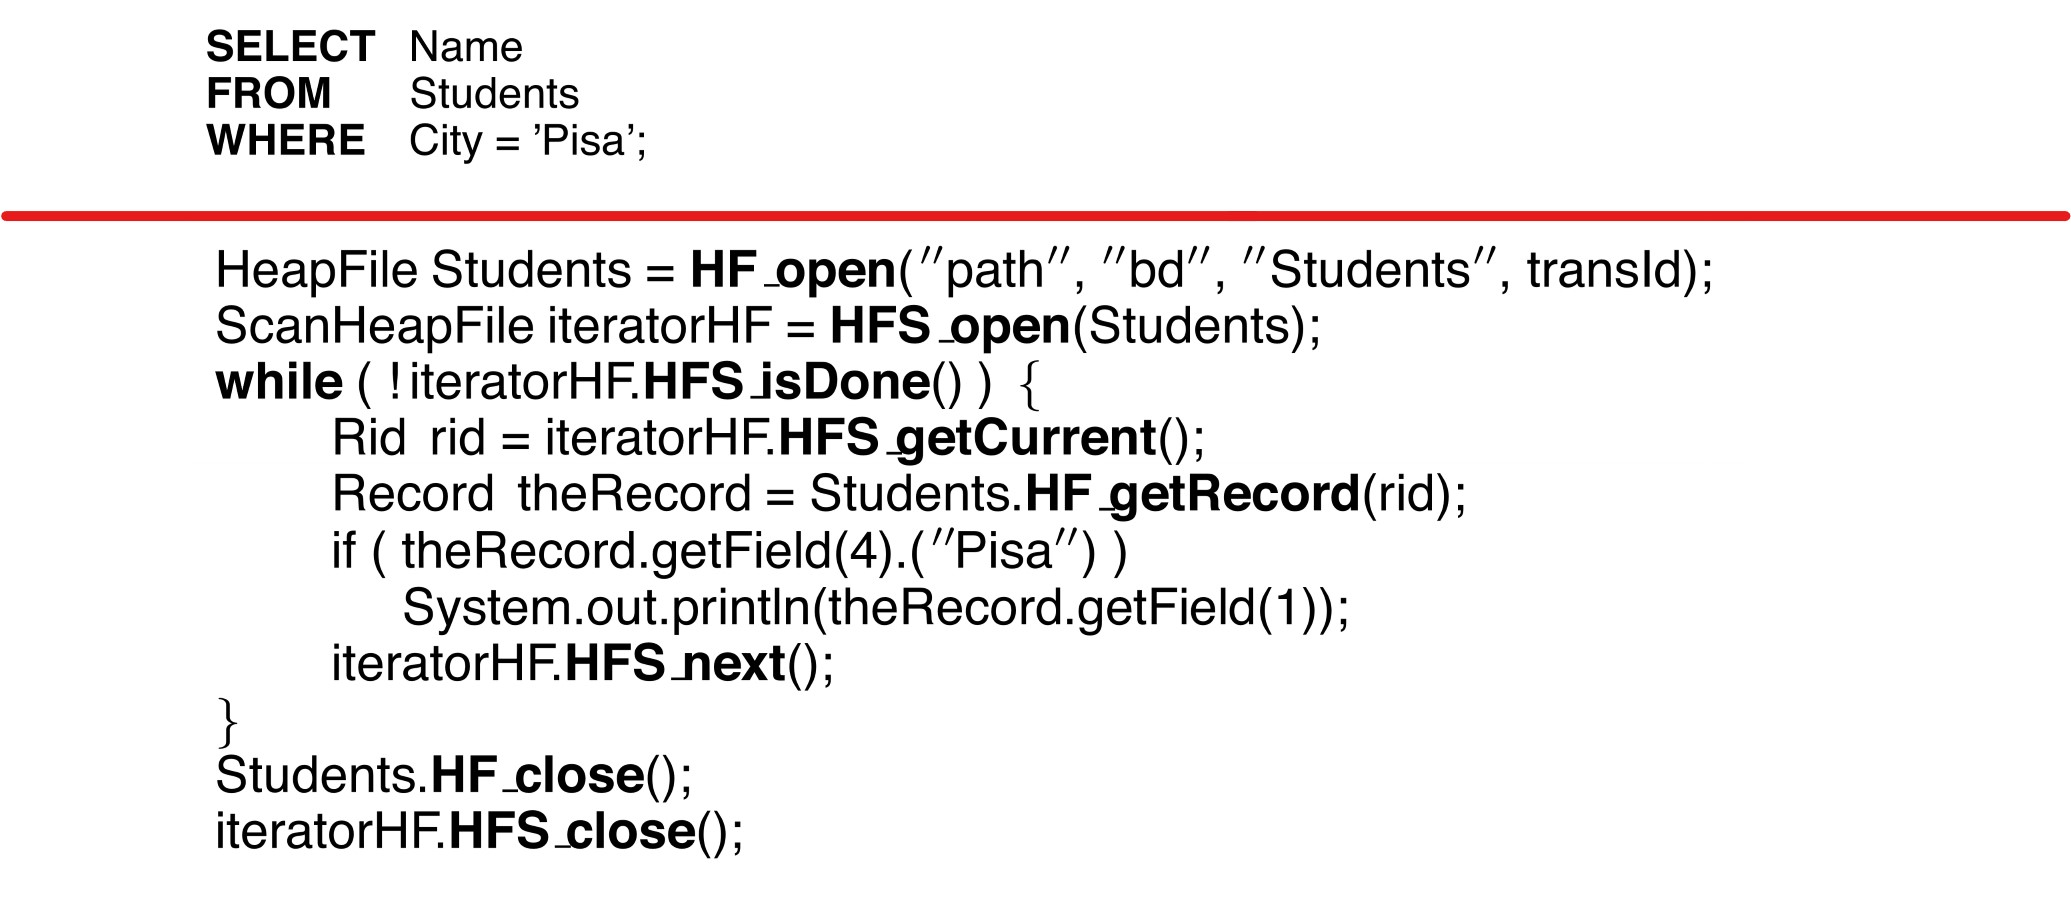
\includegraphics[scale = 0.7]{img/access2.jpg}
		\label{access2}
        \caption{Example of query plan with heap files}
\end{figure}

\begin{figure}[h!]
		\centering
		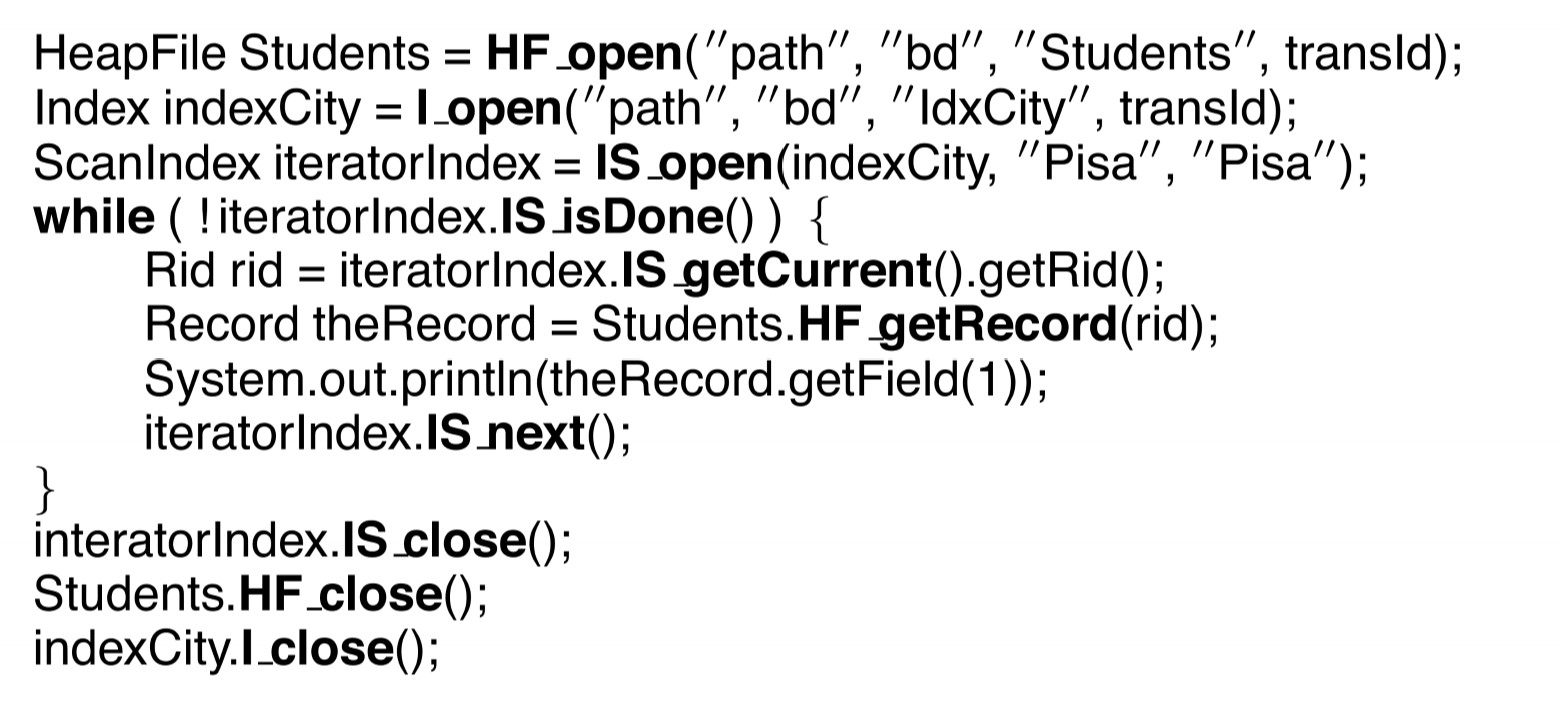
\includegraphics[scale = 0.7]{img/access3.jpg}
		\label{access3}
        \caption{Example of query plan with indexes}
\end{figure}